\section{Scelte di progettazione}
Partendo dal final-term sono state eseguite differenti modifiche ai vari contratti, sia alla struttura del progetto stesso. I contratti scritti in \textit{Solidity} sono adesso 3: \texttt{EnglishAuction}, \texttt{VicreyAuction} e \texttt{AuctionManager}. Quest'ultimo è stato inserito per gestire la creazione, la distruzione delle varie aste da parte degli utenti e per dare un punto di riferimento per l'utilizzo dei contratti.\newline
L'\texttt{AuctionManager} è il contratto che viene caricato all'interno delle \textit{Block-chain}, all'interno sono presenti tutti gli indirizzi corrispondenti ai contratti delle aste attive. Grazie ad una variabile booleane \texttt{couldCreateAuction} è possibile impedire o consentire la creazioni delle aste, di seguito sono riportate delle brevi descrizioni dei metodi definiti:
\begin{itemize}
	\item \texttt{createEnglishAuction(...)}: se \texttt{couldCreateAuction == true}, crea una nuova istanza di un contratto \texttt{EnglishAuction}, chiamando il suo costruttore e salvandone l'indirizzo;
	\item \texttt{createVicreyAuction(...)}: se \texttt{couldCreateAuction == true}, crea una nuova istanza di un contratto \texttt{VicreyAuction}, chiamando il suo costruttore e salvandone l'indirizzo;
	\item \texttt{deleteEnglishAuction(...)}: rimuove un indirizzo dalle aste \texttt{EnglishAuction} salvate, questa funzione è di tipo \texttt{internal} (può essere richiamata solo da altri contratti);
	\item \texttt{deleteVicreyAuction(...)}: rimuove un indirizzo dalle aste \texttt{VicreyAuction} salvate,  questa funzione è di tipo \texttt{internal} (può essere richiamata solo da altri contratti);
	\item \texttt{getAllAuctions()}: restituisce tutte le aste attive in due array di indirizzi;
	\item \texttt{stopCreation()}: se \texttt{couldCreateAuction == true}, lo pone a \texttt{false};
	\item \texttt{startCreation()}: se \texttt{couldCreateAuction == false}, lo pone a \texttt{true};
	\item \texttt{destroyManager()}: se non vi sono aste attive, chiama il metodo \texttt{selfDestruct}.
\end{itemize}
LA flag \texttt{couldCreateAuction} è stata pensata per permettere al "manager" di fermare le future creazioni di aste, in modo tale da poter richiamare il metodo \texttt{selfDestruct} senza perdere riferimenti ad aste attive. Infatti, per poter interagire con le varie aste tramite la \textbf{DAPP} sviluppata, occorrono gli indirizzi salvati all'interno del contratto "manager".\newline
\begin{figure}[h]
	\centering
	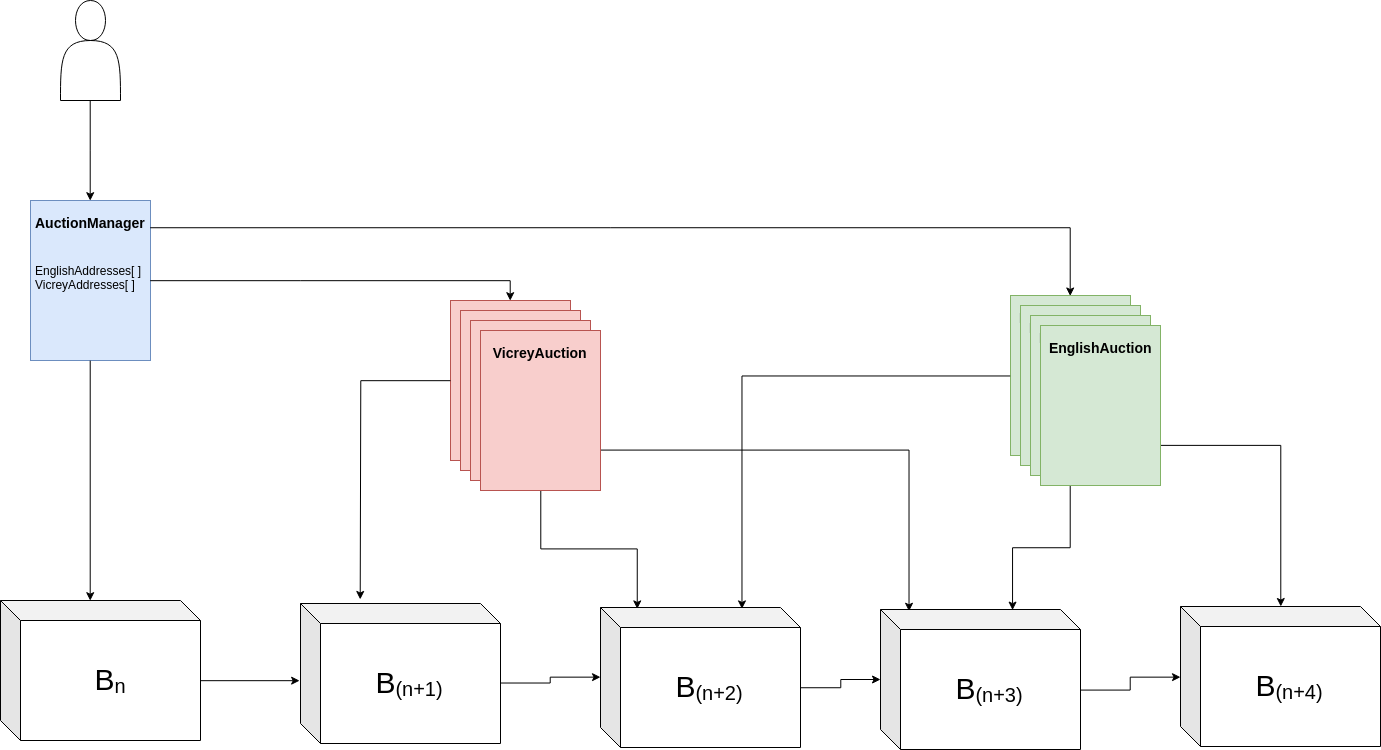
\includegraphics[scale=0.3]{contratti.png}
	\caption{Diagramma della struttura dei contratti.}\label{fig1.1}
\end{figure}\newline
Questo sistema garantisce che, l'unico indirizzo che occorre salvare all'interno di un server (lo stesso server che fornisce il codice della \textbf{DAPP}) sarà quello dell'\texttt{AuctionManager}, aumentando così la sicurezza dell'applicazione. Inoltre, il "manager" si fa carico della consistenza delle aste e dei pagamenti. All'interno dei contratti \texttt{EnglishAuction} e \texttt{VicreyAuction} è stata infatti aggiunta una fase dopo la finalizzazione dell'asta. In quest'ultima fase, il pagamento del vincitore viene "congelato" nel deposito del contratto stesso, permettendo all'utente di ricevere il bene prima di estinguere il pagamento (un po' come funziona PayPal). Nel caso in cui però, il vincitore non dovesse estinguere il pagamento anche dopo aver ricevuto il bene, il "manager" (i.e. l'account che ha instanziato il contratto \texttt{AuctionManager}) può estinguere egli stesso il pagamento nel caso in cui sia passato un sufficiente lasso di "tempo" (per la precisione si parla di numero blocchi minati, tale periodo è stato impostato a 1440 blocchi, circa 5 giorni).\newline
Inoltre, l'\texttt{AuctionManager}) può eventualmente cambiare la fase delle aste. Le fasi vengono scandite dal trascorrere dei blocchi, ogni 5 blocchi la fase \textbf{puo'} cambiare, ma essa non cambia fintanto che qualcuno non interagisce con il contratto. Ogni funzione infatti include un \texttt{modifier} che controlla se siano passati o meno 5 blocchi dall'ultimo cambio di fase e, in caso affermativo, passa alla fase successiva (in particolare ciò non avviene nelle fasi di \texttt{finilizing} e \texttt{pending}). Il venditore dell'asta (i.e. l'account che l'ha creata) però può richiamare la funzione \texttt{nextPhase} per cambiare manualmente fase, sempre rispettando il periodo dei 5 blocchi. Potrebbe accadere che se nessuno fosse interessato all'asta anche il venditore potrebbe non interagire più con il contratto e lasciare che esso non venga mai distrutto. Perciò, anche il "manager" ha la possibilità di cambiare manualmente fase attraverso la stessa funzione.\newline
Infine si è deciso di utilizzare un server MySql per salvare "Titolo" e "Descrizione" delle varie aste. Utilizzare direttamente i contratti per salvare stringhe di grande dimensioni è costoso in quanto l'utilizzo efficiente e minimale della memoria all'interno della blockchain è una proprietà fondamentale per lo sviluppo di un buon SmartContract, in quanto l'operazione associata allo \texttt{STORAGE} di variabili in memoria è la più costosa di tutte. Da un punto di vista della sicurezza, questa decisione non implica nessuna minaccia in quanto "attaccare" il database per modificarne le informazioni salvate al suo interno, non produrrebbe alcun effetto sulla blockchain e potrebbe essere facilmente individuato e corretto.
\section{Scelte implementative}
\subsection{Contratto AuctionManager}
Nel particolare nel contratto \texttt{AuctionManager}) si è scelto di salvare gli indirizzi delle aste attiva tramite l'utilizzo di un \texttt{mapping} (usando come chiavi l'indirizzo del contratto) e di un \texttt{array} di supporto. La prima viene utilizzata per controllare l'esistenza di un dato indirizzo all'interno di quelli attivi, in modo da avere un accesso a costo unitario. L'\texttt{array} viene invece utilizzato laddove è necessario usare l'indirizzo stesso del contratto, infatti in \texttt{Solidity} non è possibile accedere alle chiavi di un \texttt{mapping}. Visto questo tipo di struttura, quando occorre eliminare un'asta dal contratto "manager" è necessario spostare l'ultimo elemento dell'\texttt{array} nella posizione lasciata vuota dall'elemento eliminato e , soprattutto, bisogna diminuire la lunghezza dell'\texttt{array}. Gli \texttt{array} dinamici, infatti, mantengono la proprio dimensione anche dopo aver chiamata la funzione \texttt{delete} sul l'elemento specificato, portando a comportamenti indesiderati soprattutto nel caso in cui si vogliano accedere gli elementi nelle utlime posizioni.\newline
\subsection{DAPP}
Per lo sviluppo della DAPP, sono stati necessari diversi FrameWork e libreria in modo da impostare tutto l'environment necessario per testare e implementare sia i contratti che la DAPP stessa. Per la precisione si è fatto uso di:\newline
\begin{itemize}
 	\item \textbf{Truffle}: un FrameWork necessario a testare e deployare i contratti;
 	\item \textbf{Web3}: una libreria necessaria per interagire tramite javascript con i contratti sulla blockchain;
 	\item \textbf{Truffle-contracts}: una libreria simile a Web3, con qualche funzionalità in meno, rende l'interazione con i contratti più semplice ed intuitiva;
 	\item \textbf{NodeJS}: un FrameWork utilizzato per gestire la DAPP sviluppata in javascript e jquery, e per interagire con Truffle;
 	\item \textbf{lite-server}: una libreria utilizzata come server per "servire" la DAPP e i suoi moduli;
 	\item \textbf{bn.js}: una libreria in javascript necessaria a manipolare i valori dei numeri utilizzati dai contratti della blockchain (e.g. uint256, o valori in Wei), evitando errori di integer overflow e di precisione;
 	\item \textbf{MetaMask}: un'estensione del browser che permette di collegarsi ai nodi della blockchain, in modo da poter interagire con diverse blockchain sia di testi che reali;
 	\item \textbf{Ganache-cli}: una blockchain locale di testing, permette di simulare una vera rete su cui è possibile deployare e conseguentemente interagire con i contratti scritti in Solidity;
 	\item \textbf{Boostrap}: una serie di librerie di stile CSS e javascript per renderizzare la DAPP;
 	\item \textbf{Express} : una libreria javascript server-side per salvare i dati delle aste quali "titolo" e "descrizione" in un server MySql;
 	\item \textbf{Truffle-assertion} : una libreria di NodeJS per testare i contratti.
\end{itemize}
\begin{figure}[h]
	\centering
	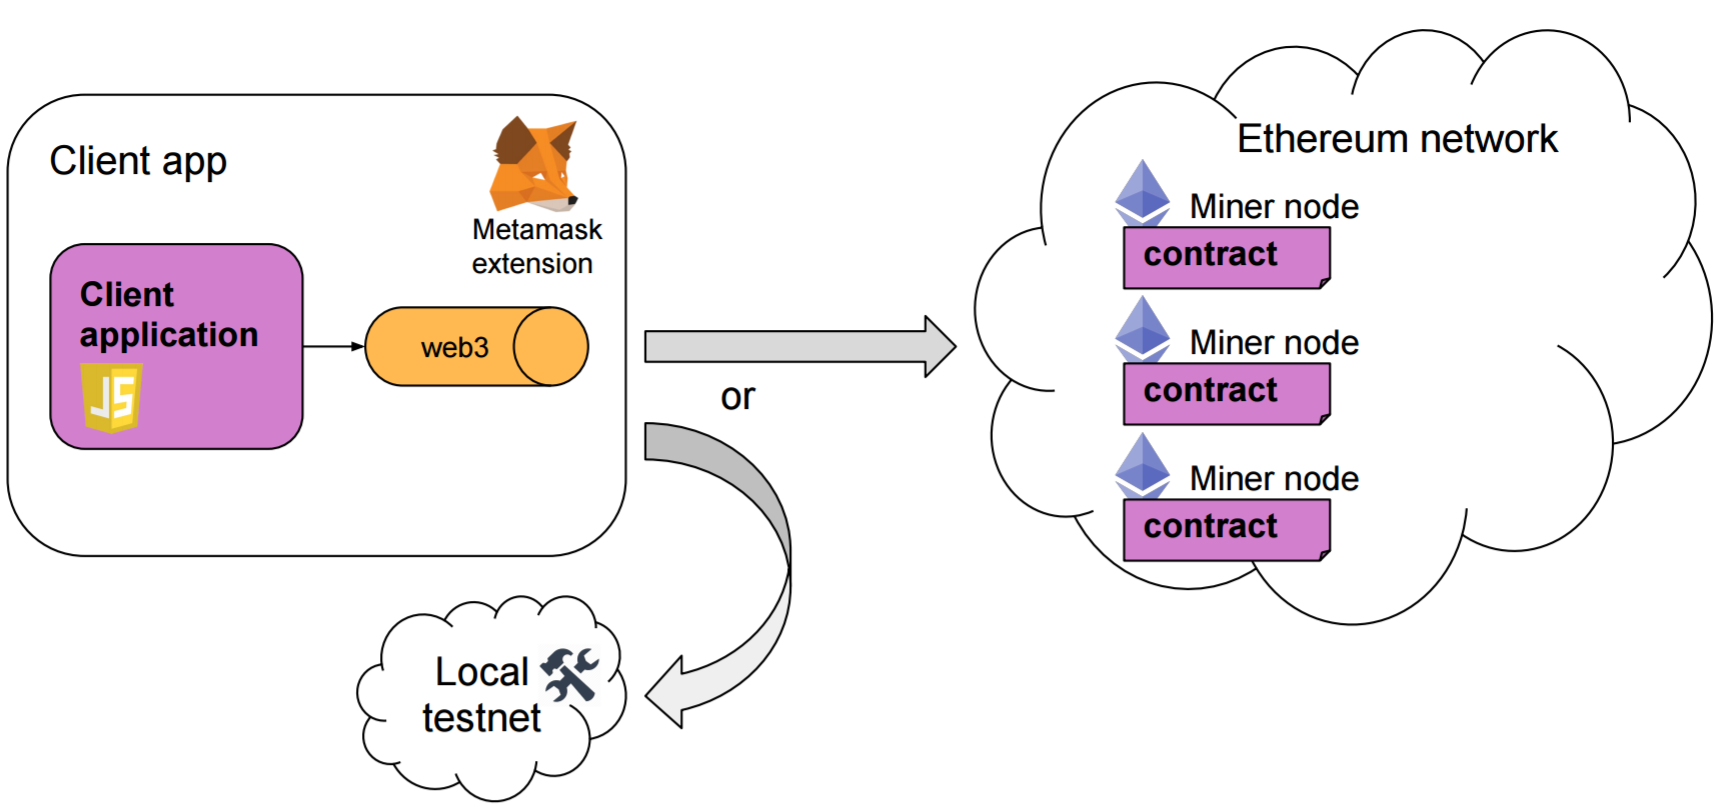
\includegraphics[scale=0.3]{suite.png}
	\caption{Environment parziale per interfacciarsi al mondo delle blockchain.}\label{fig1.2}
\end{figure}
Prima di illustrare il funzionamento della DAPP nello specifico, vanno fatte alcune considerazioni sul "versioning" delle varie parti utilizzate per il suo sviluppo. In particolare la versione di Web3 utilizzata è la 1.0.0.beta37, essendo una versione in via di sviluppo non tutti i metodi funzionano correttamente soprattutto dato che l'environment necessario è composto da un grande numero di FrameWork e libreria che devono interagire tra loro.\newline
La DAPP si presenta divisa in tre sezione, una per tipologia di contratto (i.e. \texttt{EnglishAuction}) e \texttt{VicreyAuction}) più una sezione che varia a seconda di quale sia l'account di MetaMask utilizzato per collegarsi alla DAPP. Nel caso in cui si connetta con l'indirizzo "manager" verranno mostrati tutti i contratti salvati all'interno del'\texttt{AuctionManager}) (nelle rispettive sezioni) che si trovano nella fase di "Pending" e in più verranno mostrati tutti quei contratti in cui la fase non cambia da più di 546 blocchi (i.e. circa 2 giorni). In questo modo al "manager" verranno mostrati solo i contratti di vero interesse e non tutti gli altri (con cui nello specifico non può interagire se non per far progredire la fase). La terza sezione comprende alcune utilità che permettono al "manager" di bloccare la creazione di altre aste e in caso di distruggere il contratto stesso.\newline
Se invece ci si connette con un account qualsiasi che ha o meno interagito con i vari contratti già "deployati", le prime due sezioni mostreranno tutti i contratti con cui l'utente puòà interagire, mostrando le varie fasi in cui essi si trovano. Nello specifico verranno mostrati quei contratti che seguono le seguenti specifiche:\newline
\texttt{EnglishAuction}:
\begin{itemize}
	\item Fase = \textbf{Glory Phase}, l'utente può comprare il bene prima dell'inizio dell'asta;
	\item Fase = \textbf{Glory Phase}, ma sono passati più di 5 blocchi dall'ultimo cambio di fase, l'utente non può comprare il bene ma può sottomettere una puntata (cambiando di conseguenza la fase tramite il \texttt{modifier});
	\item Fase = \textbf{Submitting Phase}, l'utente può sottomettere la sua puntata;
	\item Fase = \textbf{Submitting Phase}, ma sono passati più di 5 blocchi dall'ultimo cambio di fase, in questo caso tale asta verrà mostrata se e solo se l'utente è il vincitore dell'asta. In tal caso avrà la possibilità di finalizzare l'asta, passando automaticamente alla fase successiva;
	\item Fase = \textbf{Finilizing Phase}, se e solo se l'utente è il vincitore dell'asta, permettendogli di finalizzare l'asta;
	\item Fase = \textbf{Pending Phase}, se e solo se l'utente è il vincitore dell'asta, permettendogli di estinguere il pagamento l'asta;
\end{itemize}
\texttt{VicreyAuction}:
\begin{itemize}
	\item Fase = \textbf{Glory Phase}, l'utente non può interagire con l'asta in alcun modo;
	\item Fase = \textbf{Glory Phase}, ma sono passati più di 5 blocchi dall'ultimo cambio di fase, l'utente può "committare" una puntata (cambiando di conseguenza la fase tramite il \texttt{modifier});
	\item Fase = \textbf{Committing Phase}, l'utente può "committare" la sua puntata;
	\item Fase = \textbf{Committing Phase}, ma sono passati più di 5 blocchi dall'ultimo cambio di fase, in questo caso tale asta verrà mostrata se e solo se l'utente è tra i partecipanti (i.e. ha inserito na puntata). Inoltre l'utente potrà direttamente scartare la sua puntata in quanto la fase cambierà in automatico;
	\item Fase = \textbf{Whitdrawal Phase}, se e solo se l'utente è tra i partecipanti, permettendogli di scartare la propria puntata;
	\item Fase = \textbf{Whitdrawal Phase}, ma sono passati più di 5 blocchi dall'ultimo cambio di fase, in questo caso tale asta verrà mostrata se e solo se l'utente è tra i partecipanti (i.e. non ha scartato la sua puntata), l'utente potrà quindi aprire la sua puntata;
	\item Fase = \textbf{Opening Phase}, se e solo se l'utente è tra i partecipanti, permettendogli di aprire la propria puntata;
	\item Fase = \textbf{Opening Phase}, ma sono passati più di 5 blocchi dall'ultimo cambio di fase, in questo caso tale asta verrà mostrata se e solo se l'utente è il vincitore dell'asta, permettendogli di finalizzarla;
\end{itemize}
Le ultime due fasi sono equivalenti al caso dell'\texttt{EnglishAuction}. Inoltre, le aste di cui l'utente è il venditore, mostreranno sempre un pulsante per cambiare fase (disabilitato nel caso in cui non sia passato il tempo necessario), permettendogli inoltre di finalizzare l'asta (senza cambiare fase) se si trovasse nella dase di Opening Phase al momento giusto. L'ultima sezione invece comprende un form per creare una nuova asta, di qualsiasi tipo, per mettere in vendita un qualunque bene.\newline
Tutte le istanze dei contratti che vengo visualizzate nella DAPP (e.g. quelle con cui l'utente può interagire), si sottoscrivono a tutti gli eventi di interesse che portino a cambiare lo stato dell'asta stesso (e.g. cambio di fase, sottomissione di una puntata più alta, finalizzazione o estinzione di un asta di cui l'utente è proprietario etc...). Inoltre ogni asta può essere aggiornata singolarmente tramite un apposito pulsante che ne ricarica le varie informazioni.
\section{Testing}
\subsection{Test Contratti}
Per testare i contratti sono stati scritti dei test specifici con Truffle in cui vengono testate alcune situazioni particolari. Per \texttt{EnglishAuction} vengono eseguiti 4 test specifici:
\begin{itemize}
	\item "Test \_Buy Out the good": si eseguono una serie di transazioni per comprare il bene prima che cominci l'asta;
	\item "Test \_Making a bid": si eseguono una serie di transazioni per eseguire una puntata durante l'asta;
	\item "Test \_Same address 2 bids \_A lower bid!": prima si cerca di fare due puntate dallo stesso account, poi si cerca di fare una puntata più bassa di quella attualmente vincente;
	\item "Test \_No bids": si crea e conclude l'asta senza fare alcuna puntata;
\end{itemize}
Per \texttt{VicreyAuction} vengono i seguenti test:
\begin{itemize}
	\item "Test \_deposit transaction": si esegue un withdraw e si controllo che venga perso metà del deposito;
	\item "Test \_Highest Bid and Second highest must change": si eseguono una serie di transazioni per arrivare alla fase di opening e controllare che sia il primo che il secondo vengano aggiornati correttamente;
	\item "Test \_No bids": si crea e conclude l'asta senza fare alcuna puntata;
\end{itemize}
Per eseguire tali test è stato utilizzato Ganache con la funzione di "automining" attiva, la fase è stata controllata e fatta avanzare tramite un ciclo while richiama la fase del contratto. I test infatti risultano essere lenti, soprattutto è necessario impostare l'automining al di sopra dei 5 secondi per non incorrere in errori.\newline
Il contratto \texttt{AuctionManager} è stato invece testato direttamente sulla DAPP in quanto non presenta particolari casistiche.
\subsection{Test DAPP}
Per eseguire un test sul funzionamento della DAPP occore installare MetaMask nel browser e lanciare sia lite-server (port:3000) che express (port:5000). Dall'icona di MetaMask è possibile selezionare la network di testing (port:8545) che viene emulata ancora una volta con Ganache. Per far si che MetaMask si connetta ad un account della block chain, è necessario copiare uno degli indirizzi che Ganache mette a disposizione (il numero 3 è stato utilizzato come predefinito) e copiare Api key all'interno di MetaMask. Inoltre, è necessario deployare i contratti, a tal proposito, nel file \texttt{truffle-config.json} sono state definite due network. La prima è quella utilizzata per i test su Ganache, la seconda viene utilizza per la connessione alla block chain di test di Ropsten. Per deployare il contratto manager e eseguire la Dapp, è necessario eseguire i seguenti comandi in terminali diversi (di cui gli ultimi due vanno eseguiti nella cartella contenete il progetto, mentre il primo va eseguito dopo aver lanciato il server MySql nella cartella contente il server in Express):
\begin{verbatim}
$ npm start
$ ganache-cli -p 8545 -b 5 -l 0x1ffffffff
$ truffle migrate --reset --network  development
$ npm run dev
\end{verbatim}
Il flag "network" indica su quale rete verrà eseguito il file di "migrazione" dei contratti. Nel file \texttt{2\_deploy\_contracts.js} sono definiti i vari comandi per deployare i diversi contratti a seconda della rete in cui ci si trova. Quindi connettendosi a Ganache verranno istanziati diversi contratti per popolare appropriatamente la DAPP durante il test. In particolare si consiglia di configurare MetaMask con l'account numero 3, o con il numero 0 se si vuole vedere l'interfaccia dal punto di vista del manager. Non essendo necessario un login per diversificare gli account in quanto già lo sono, occorre settarli manualmente all'interno di MetaMask.
\subsection{Test Ropsten}
Infine il progetto è stato testato anche su Ropsten, con qualche difficoltà iniziale, utilizzando come nodo di accesso Infura. Basterà eseguire lo stesso comando visto in precedenza senza la flag \texttt{--reset} e con la giusta network. Non è stato possibile eseguire molti test su tale rete in quanto non si posseggono lo stesso numero di account che offre Ganache e tanto meno lo stesso ammontare di Ether. In ogni contratto inoltre è raggiungibile un metodo di \texttt{selfdestruct} per evitare di lasciare contratti svincolati sulla network pubblica.